% =====================================================================
% MSc Project Proposal -- Kingston University
% Strengthening User Privacy through AI-Driven Risk Quantification
% and International Standards Alignment
% Author: Jay Bell  (K2119852)
% =====================================================================
\documentclass[12pt,a4paper,titlepage]{article}

% --- BASIC ENCODING & LANGUAGE ---
\usepackage[utf8]{inputenc}
\usepackage[T1]{fontenc}
\usepackage[english]{babel}

% --- FONT (Times New Roman) & SPACING ---
\usepackage{mathptmx}
\usepackage[onehalfspacing]{setspace}
\usepackage{footmisc}
\renewcommand{\footnotelayout}{\fontsize{10}{12}\selectfont}

% --- PAGE MARGINS ---
\usepackage[a4paper,left=2cm,right=2cm,top=2cm,bottom=2cm,bindingoffset=5mm]{geometry}

% --- MATH ---
\usepackage{amsmath, amssymb}
\usepackage{bm}
\usepackage{amsthm}

% --- IMAGES & TABLES ---
\usepackage{graphicx}
\graphicspath{{./images/}}
\usepackage{booktabs}
\usepackage{tabularx}
\usepackage{multirow}
\usepackage{float}
\usepackage{caption}
\usepackage{subcaption}
\usepackage{array}

% --- LISTS ---
\usepackage{enumitem}

% --- DIAGRAMS / GANTT ---
\usepackage{tikz}
\usetikzlibrary{shapes.geometric, arrows.meta, positioning, fit, backgrounds}
\usepackage{pgfgantt}

% --- UTILITIES ---
\usepackage{xcolor}
\usepackage[plainpages=false, hidelinks]{hyperref}
\usepackage{cleveref}
\usepackage[verbose]{placeins}
\usepackage{appendix}

% --- equation autoref tweak (kept from supplied template) ---
\makeatletter
\def\tagform@#1{\maketag@@@{\ignorespaces#1\unskip\@@italiccorr}}
\let\orgtheequation\theequation
\def\theequation{(\orgtheequation)}
\makeatother
\let\orgautoref\autoref
\providecommand{\Autoref}[1]{\def\equationautorefname{Equation}\orgautoref{#1}}
\renewcommand{\autoref}[1]{\def\equationautorefname{Eq.}\orgautoref{#1}}

% --- BIBLIOGRAPHY ---
\usepackage{csquotes}
\usepackage[backend=biber, style=authoryear, sorting=nyt, maxcitenames=2, maxbibnames=99]{biblatex}
\addbibresource{references.bib}

\setcounter{tocdepth}{2}

% --- DOCUMENT INFO ---
\title{Strengthening User Privacy through AI-Driven Risk Quantification and International Standards Alignment}
\author{Jay Bell}
\date{30 June 2026}

% =========================================
\begin{document}
% =========================================

% --- Title Page ---
\begin{titlepage}
    \begin{center}
        \par
        \vspace*{1.5cm}
        {\large \textsc{Kingston University -- Faculty of Engineering, Computing and the Environment}}
        \par
        \vspace{2.5cm}
        {\LARGE \textbf{Strengthening User Privacy through\\[0.4em]
        AI-Driven Risk Quantification and\\[0.4em]
        International Standards Alignment}}
        \par
        \vspace{1.5cm}
        {\large MSc Project Proposal}
        \par
        \vspace{3cm}
        {\textsc{A proposal presented to the School of Computer Science and Mathematics in partial fulfilment of the requirements for the degree of}}\\[0.6em]
        {\textsc{Master of Science in Artificial Intelligence}}
        \par
        \vspace{3cm}
        {\textsc{Supervisor:} Arshad Razi}\\[0.4em]
        \vspace{1cm}
        {\textsc{Submitted on 30 June 2026 by}\\[0.3em]
        Jay Bell\\[0.2em]
        Student ID: K2119852}\\
    \end{center}
\end{titlepage}
\thispagestyle{empty}

\pagenumbering{roman}
\newpage
\tableofcontents
\newpage
\listoffigures
\addcontentsline{toc}{section}{List of Figures}
\newpage
\listoftables
\addcontentsline{toc}{section}{List of Tables}
\newpage

\cleardoublepage
\pagenumbering{arabic}
\setcounter{page}{1}

% =====================================================================
\section*{Abstract}
\addcontentsline{toc}{section}{Abstract}
% =====================================================================

User privacy is increasingly regulated by international standards and legal instruments, yet existing artificial intelligence (AI) tools that analyse privacy policies remain disconnected from these standards and produce no quantitative, interoperable indicators of risk. This proposal sets out a five-month MSc project that addresses this gap by developing an AI-driven framework for quantifying user privacy risk in line with ISO/IEC, NIST, IEEE and GDPR requirements. The project will (i) translate selected standards clauses into measurable indicators, (ii) define multi-level metrics across user, system and organisation views, (iii) combine a fine-tuned PrivacyBERT clause classifier with a Bayesian probabilistic risk model, and (iv) validate the prototype on synthetic logs and public breach datasets (ENISA, Privacy Rights Clearinghouse). The output is a validated proof-of-concept tool, a draft metric set, and a roadmap towards a fuller standards-aligned framework. Initial work in the supporting repository, including standards-to-control extraction and a reproducible Phase~3 freeze, demonstrates the technical feasibility of the proposed plan.

% =====================================================================
\section{Introduction and Background}\label{sec:intro}
% =====================================================================

The protection of personal data has become a defining technical and regulatory concern of the past decade. Regulators in the European Union, the United Kingdom and the United States have responded with overlapping but heterogeneous instruments, including the General Data Protection Regulation \parencite{gdpr2016}, the NIST Privacy Framework \parencite{nist_pf_2020}, the family of ISO/IEC 27000-series standards \parencite{iso27001_2022, iso27701_2019, iso29100_2011, iso29151_2017}, and most recently the EU AI Act \parencite{eu_ai_act_2024}. These instruments place increasing pressure on \emph{measurable} privacy assurance: not only that controls exist, but that their effectiveness can be evaluated and compared.

The stakeholders affected are diverse. \textbf{Data subjects} need understandable, comparable indicators of how a given service treats their information. \textbf{Data controllers and processors} must demonstrate compliance to auditors and regulators, often across several overlapping standards simultaneously. \textbf{Regulators and auditors} need objective evidence to support enforcement decisions. \textbf{Researchers} require reproducible benchmarks for new privacy-preserving techniques. Each of these stakeholders is currently underserved.

The core problem this project addresses is the disconnect between two communities of work. On one side, AI-based privacy-policy analysis tools such as Polisis \parencite{harkous2018polisis} and PrivacyBERT-LSTM \parencite{muralitharan2024privacybertlstm} can classify clauses with high accuracy but stop short of producing standards-aligned, quantitative risk scores. On the other side, standards and regulatory frameworks define rich principles (consent, data minimisation, purpose limitation, encryption, third-party sharing) but provide no operational metrics to evaluate them at scale. The recent IEEE survey by \textcite{arshad2024characterisation} confirms that no current approach integrates AI-driven privacy analysis with standards-based compliance measurement, and identifies multi-level quantification as an open challenge.

The project is important because measurable privacy risk underpins three concrete benefits. For data subjects, comparable scores improve transparency and informed consent. For organisations, multi-level metrics support targeted remediation and reduce audit cost. For regulators, calibrated risk indicators enable evidence-based enforcement and post-incident analysis using public breach corpora such as ENISA's Threat Landscape \parencite{enisa_tl_2024} and the Privacy Rights Clearinghouse chronology \parencite{prc_breaches}.

Building on prior work, the project takes existing strengths --- transformer-based clause classification, probabilistic risk modelling and standards taxonomies --- and integrates them into a single multi-level pipeline. The central research question is therefore: \emph{To what extent can a transformer-based clause classifier, coupled with a Bayesian probabilistic scorer and a clause-to-standard traceability map, produce calibrated, multi-level privacy-risk indicators that align with ISO/IEC, NIST and GDPR requirements?}

% =====================================================================
\section{Aims and Objectives}\label{sec:aims}
% =====================================================================

\paragraph{Overall aim.}
To design, implement and validate an AI-driven, standards-aligned framework for quantifying user privacy risk that combines transformer-based clause classification with Bayesian probabilistic scoring, evaluated against synthetic and publicly available breach data.

\paragraph{Objectives.} The aim is decomposed into five SMART objectives. The annotations \emph{(S, M, A, R, T)} indicate, respectively, that each objective is \emph{specific}, \emph{measurable}, \emph{achievable}, \emph{relevant} to the MSc programme, and \emph{time-bound}.

\begin{description}[leftmargin=1.6em,style=nextline]
    \item[\textbf{O1 -- Standards-to-metrics mapping.}]
        Extract candidate privacy controls from at least four standards families (GDPR, ISO/IEC 27001/27701/29100/29151, NIST Privacy Framework, NIST AI RMF) and map them to a normalised indicator catalogue.
        \emph{(S)} Targets a defined corpus of clauses; \emph{(M)} success measured by traceability coverage (\(\geq 90\%\) of selected clauses mapped to at least one indicator); \emph{(A)} achievable using existing parsers and the standards corpus already in the project repository; \emph{(R)} provides the foundation for all later phases; \emph{(T)} delivered by end of Month~1 (28 February 2026).

    \item[\textbf{O2 -- Multi-level metric definition and synthetic data.}]
        Specify metric formulas at user, system and organisation levels, generate a synthetic event dataset and run baseline scoring.
        \emph{(S)} Three explicit metric levels with documented formulas; \emph{(M)} baseline scoring produces interpretable distributions on at least 1{,}000 synthetic events; \emph{(A)} reuses Phase~1 indicator catalogue; \emph{(R)} supports validation in later phases; \emph{(T)} delivered by end of Month~2 (31 March 2026).

    \item[\textbf{O3 -- Clause classification model.}]
        Fine-tune a PrivacyBERT-style transformer on the OPP-115 corpus \parencite{wilson2016opp115, opp115_dataset} and Polisis-derived data, achieving competitive classification performance on the standard categories.
        \emph{(S)} Targets the 10 OPP-115 high-level categories; \emph{(M)} macro-F1 \(\geq 0.70\) on a held-out test split, with calibration reported; \emph{(A)} achievable on a single CUDA-class GPU; \emph{(R)} produces clause-level evidence consumed by O4; \emph{(T)} delivered by end of Month~3 (30 April 2026).

    \item[\textbf{O4 -- Bayesian risk integration.}]
        Combine clause classifier outputs with a Bayesian probabilistic risk model that scores user-, system- and organisation-level risk using the Phase~2 metrics.
        \emph{(S)} A single risk pipeline with documented inputs/outputs; \emph{(M)} produces calibrated posterior distributions and bootstrap confidence intervals on a held-out evaluation set; \emph{(A)} builds on \texttt{pgmpy}-style toolkits and the existing Phase~3 freeze; \emph{(R)} addresses the core research question; \emph{(T)} delivered by mid-Month~4 (15 May 2026).

    \item[\textbf{O5 -- Validation, benchmarking and final report.}]
        Benchmark the prototype against defined metrics on real and synthetic data and deliver a validated tool plus the final MSc report.
        \emph{(S)} Validation report comparing the integrated model against logistic-regression and naive-Bayes baselines; \emph{(M)} statistically significant improvement on at least one calibration metric (Brier score or ECE) with bootstrap CIs; \emph{(A)} ablation pipelines already exist in the project repository; \emph{(R)} satisfies MSc assessment criteria; \emph{(T)} final submission on 30 June 2026.
\end{description}

Intermediate, enabling deliverables include a reproducible build pipeline, a unit-test suite covering parsers and chunking, and a small Gradio demonstration interface for the validation phase.

% =====================================================================
\section{Literature Review}\label{sec:litrev}
% =====================================================================

The proposed framework sits at the intersection of four research strands: privacy-policy natural language processing (NLP), privacy quantification and breach analytics, standards and regulatory frameworks, and probabilistic risk modelling. This review summarises and critiques each strand, then identifies the gap that motivates the project.

\subsection{AI for privacy-policy analysis}

A first generation of work focused on automatically classifying privacy-policy clauses. The OPP-115 corpus introduced by \textcite{wilson2016opp115} provides 115 manually annotated policies across ten high-level data-practice categories and remains the de-facto benchmark for the field. Building on this, \textcite{harkous2018polisis} introduced \emph{Polisis}, a hierarchical neural classifier that demonstrated the feasibility of large-scale automated policy analysis and powers downstream tools such as PriBot. More recently, \textcite{muralitharan2024privacybertlstm} proposed a PrivacyBERT-LSTM hybrid that improves on earlier baselines for sensitive-information detection by combining transformer encoders with sequence modelling. These approaches all benefit from the broader maturation of contextual language models, particularly BERT \parencite{devlin2019bert}.

The shared limitation of this strand is scope. The output is invariably a categorical label or a per-clause probability; none of these systems produce a \emph{calibrated} risk score, nor do they trace clauses back to specific standards or regulatory obligations. As a result, their outputs are useful for transparency tools but not directly consumable by auditors or by quantitative risk frameworks.

\subsection{Privacy quantification and breach analytics}

The second strand attempts to quantify privacy at the level of users, systems or organisations. The recent IEEE survey by \textcite{arshad2024characterisation} provides the most comprehensive synthesis to date, cataloguing dozens of candidate metrics and noting that the field remains fragmented across academic communities (k-anonymity-style metrics in databases, differential privacy in statistics, risk indicators in cyber-security). Empirical breach studies, in turn, draw on data from ENISA's Threat Landscape \parencite{enisa_tl_2024} and the Privacy Rights Clearinghouse chronology \parencite{prc_breaches} to characterise incident frequency and severity. \textcite{solove2006taxonomy} provides the conceptual taxonomy of privacy harms that underpins much of this measurement work.

The critique here is twofold: existing quantification work tends to operate at a single level of abstraction (user \emph{or} organisation), and it rarely connects measurement to standards-defined obligations. Breach datasets are valuable but inherently retrospective; they describe failures rather than the latent risk profile of a system in operation.

\subsection{Standards and regulatory frameworks}

A third body of literature codifies privacy as obligations rather than measurements. The GDPR \parencite{gdpr2016} introduced principles such as data minimisation, purpose limitation and lawfulness as binding requirements. The ISO/IEC family \parencite{iso27001_2022, iso27701_2019, iso29100_2011, iso29151_2017} translates these principles into auditable controls, while the NIST Privacy Framework \parencite{nist_pf_2020} and the NIST AI Risk Management Framework \parencite{nist_aiRMF_2023} offer outcome-oriented profiles that complement ISO's control-based view. The EU AI Act \parencite{eu_ai_act_2024} extends the regulatory perimeter to algorithmic systems themselves.

These instruments are normatively rich but operationally ambiguous: ``appropriate technical and organisational measures'' (GDPR Art.~32) is not directly measurable. Bridging the gap between normative obligations and quantitative indicators is precisely the task this project takes on.

\subsection{Probabilistic risk modelling}

The fourth strand is probabilistic risk modelling, dominated by Bayesian networks and related graphical models \parencite{pearl1988probabilistic, koller2009pgm}. Bayesian methods are attractive for privacy risk because they accommodate partial evidence, support hierarchical structure (user $\rightarrow$ system $\rightarrow$ organisation) and produce calibrated posteriors with explicit uncertainty. Calibration metrics such as expected calibration error (ECE), Brier score and bootstrap confidence intervals are well established in the broader machine-learning literature. Lighter alternatives such as logistic regression and naive Bayes serve as natural baselines and ablations.

\subsection{Synthesis and gap}

Across these four strands, no single piece of work integrates clause-level NLP, standards-traceable indicators and a multi-level probabilistic risk model. \textcite{harkous2018polisis} and \textcite{muralitharan2024privacybertlstm} provide classification but not quantification; \textcite{arshad2024characterisation} surveys quantification but does not deliver an implemented standards-aligned tool; standards bodies define obligations but not metrics. This proposal targets exactly that intersection, and uses the OPP-115, Polisis, ENISA and PRC datasets as evaluation substrates.

% =====================================================================
\section{Technologies and Resources}\label{sec:tech}
% =====================================================================

The project's technology choices are summarised in \autoref{tab:tech} together with the principal alternative considered for each role and the rationale for selection. The selection prioritises reproducibility, free or low-cost access for an MSc project, and compatibility with the existing project repository.

\begin{table}[hbt]
    \centering
    \caption{Key technologies and resources, with alternatives and rationale.}
    \label{tab:tech}
    \small
    \begin{tabularx}{\linewidth}{@{}l X X@{}}
        \toprule
        \textbf{Role} & \textbf{Selected} & \textbf{Alternatives considered / rationale} \\
        \midrule
        Language and core stack & Python 3.11 & Java, Go --- rejected: weaker mature NLP and probabilistic-modelling ecosystems. \\
        Clause classifier & PrivacyBERT / DistilBERT fine-tune \parencite{devlin2019bert, muralitharan2024privacybertlstm} & Full BERT-large, GPT-class APIs --- rejected: GPU/cost constraints and reduced reproducibility for closed APIs. \\
        Risk model & Bayesian network via \texttt{pgmpy} \parencite{koller2009pgm} & Logistic regression, Naive Bayes --- retained as ablation baselines rather than primary model. \\
        Vector store / retrieval & Chroma Cloud (free tier) & FAISS (local), Pinecone --- chosen for managed infrastructure and reproducibility from any machine. \\
        Datasets (training) & OPP-115 \parencite{wilson2016opp115}, Polisis-derived corpus \parencite{harkous2018polisis} & Hand-curated policy sets --- rejected: insufficient scale and inconsistent labels. \\
        Datasets (evaluation) & ENISA Threat Landscape \parencite{enisa_tl_2024}, PRC chronology \parencite{prc_breaches}, synthetic events & Single source --- rejected: insufficient diversity for cross-validation. \\
        Standards corpus & Local copies of ISO/IEC, NIST and GDPR documents \parencite{iso27001_2022, iso27701_2019, iso29100_2011, iso29151_2017, nist_pf_2020, nist_aiRMF_2023, gdpr2016} & Online lookup --- rejected: rate-limit and version drift. \\
        Compute & Local CUDA GPU (16~GB) & Cloud GPU (Colab Pro, AWS) --- retained as fallback if local compute fails. \\
        Evaluation / testing & \texttt{pytest}, scikit-learn, bootstrap CIs & Bespoke test code --- rejected: maintenance overhead. \\
        Demonstration interface & Gradio web app & Jupyter-only demo --- rejected: not stakeholder-facing. \\
        Version control / CI & Git, GitHub & Self-hosted --- rejected: marginal benefit for an MSc-scale project. \\
        \bottomrule
    \end{tabularx}
\end{table}

A high-level view of how these components interact is shown in \autoref{fig:arch}. Privacy policies are tokenised and passed to the PrivacyBERT classifier; clause-level posteriors are combined with the standards-to-indicator map and fed into the Bayesian scorer, which emits multi-level risk distributions used for benchmarking and validation.

\begin{figure}[htbp]
    \centering
    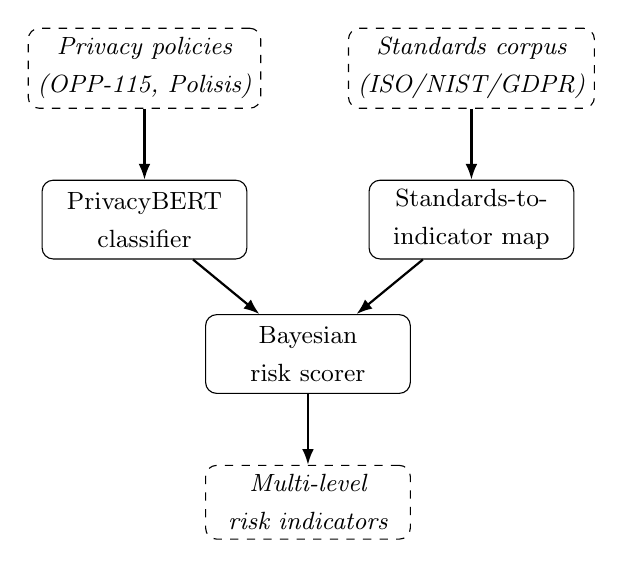
\begin{tikzpicture}[
        node distance=0.9cm and 1.1cm,
        box/.style={draw, rounded corners, minimum height=1.0cm, minimum width=2.6cm, align=center, font=\small},
        data/.style={draw, dashed, rounded corners, minimum height=0.9cm, minimum width=2.6cm, align=center, font=\small\itshape},
        arr/.style={-{Latex[length=2mm]}, thick}
    ]
        \node[data] (pol)  {Privacy policies\\(OPP-115, Polisis)};
        \node[data, right=of pol] (std)  {Standards corpus\\(ISO/NIST/GDPR)};
        \node[box, below=of pol] (bert) {PrivacyBERT\\classifier};
        \node[box, below=of std] (map)  {Standards-to-\\indicator map};
        \node[box, below=1.2cm of $(bert)!0.5!(map)$] (bayes) {Bayesian\\risk scorer};
        \node[data, below=of bayes] (out) {Multi-level\\risk indicators};
        \draw[arr] (pol)  -- (bert);
        \draw[arr] (std)  -- (map);
        \draw[arr] (bert) -- (bayes);
        \draw[arr] (map)  -- (bayes);
        \draw[arr] (bayes)-- (out);
    \end{tikzpicture}
    \caption{High-level architecture of the proposed framework.}
    \label{fig:arch}
\end{figure}

% =====================================================================
\section{Method and Work Plan}\label{sec:method}
% =====================================================================

\subsection{Research method}

The project follows a \emph{design-science research} (DSR) methodology: the central artefact is the integrated risk-quantification tool, and each phase delivers an evaluable increment. Evaluation is mixed-methods: classification quality is assessed quantitatively (macro-F1, calibration, bootstrap CIs); standards traceability is assessed qualitatively against documented clauses; end-to-end utility is assessed through a small validation study on synthetic and public breach data. Iteration between phases is explicit --- findings from validation in O5 feed back into the metric definitions of O2 and the model architecture of O3--O4.

The four phases mirror the structure already established in the supporting repository (see also \autoref{tab:artefacts} in the appendix):

\begin{enumerate}[leftmargin=1.6em]
    \item \textbf{Phase~1 (Month~1) -- Standards-to-metrics mapping.} Parse standards documents into normalised controls; chunk for retrieval; produce the indicator catalogue. \emph{Milestone~M1:} mapping artefact frozen.
    \item \textbf{Phase~2 (Month~2) -- Multi-level metrics and synthetic data.} Define formulas; generate synthetic events; run baseline scoring; partially implement organisation-level indicators. \emph{Milestone~M2:} draft metrics and synthetic dataset frozen.
    \item \textbf{Phase~3 (Month~3 -- mid-Month~4) -- Prototype build.} Fine-tune the clause classifier; integrate the Bayesian scorer; produce a reproducible \emph{freeze} bundle including LR and NB ablations. \emph{Milestone~M3:} prototype frozen.
    \item \textbf{Phase~4 (mid-Month~4 -- Month~5) -- Validation and reporting.} Benchmark on real and synthetic data; produce calibration plots and bootstrap CIs; write the final report. \emph{Milestone~M4:} validated tool and final report.
\end{enumerate}

\subsection{Schedule}

The schedule is shown in \autoref{fig:gantt}. Weekly granularity is used so that intermediate deliverables remain trackable. A thesis-writing bar overlaps Phases~3 and~4 to reflect that the report is drafted continuously.

\begin{figure}[htbp]
    \centering
    \resizebox{\linewidth}{!}{%
    \begin{ganttchart}[
        hgrid, vgrid,
        x unit=0.45cm,
        y unit chart=0.55cm,
        bar/.append style={fill=blue!30},
        bar height=.55,
        title height=1,
        milestone/.append style={fill=red!60},
        title label font=\small,
        bar label font=\small,
        milestone label font=\small\itshape,
        group label font=\small\bfseries
    ]{1}{22}
        \gantttitle{Feb 2026}{4} \gantttitle{Mar 2026}{4}
        \gantttitle{Apr 2026}{4} \gantttitle{May 2026}{5}
        \gantttitle{Jun 2026}{5}\\
        \gantttitlelist{1,...,22}{1}\\
        \ganttgroup{Phase 1: Mapping}{1}{4}\\
        \ganttbar{Standards parsing}{1}{2}\\
        \ganttbar{Indicator catalogue}{2}{4}\\
        \ganttmilestone{M1}{4}\\
        \ganttgroup{Phase 2: Metrics}{5}{8}\\
        \ganttbar{Metric formulas}{5}{6}\\
        \ganttbar{Synthetic data + baseline}{6}{8}\\
        \ganttmilestone{M2}{8}\\
        \ganttgroup{Phase 3: Prototype}{9}{14}\\
        \ganttbar{PrivacyBERT fine-tune}{9}{11}\\
        \ganttbar{Bayesian scorer}{11}{14}\\
        \ganttbar{Ablations (LR, NB)}{12}{14}\\
        \ganttmilestone{M3}{14}\\
        \ganttgroup{Phase 4: Validation}{15}{22}\\
        \ganttbar{Benchmarking}{15}{17}\\
        \ganttbar{Calibration + CIs}{16}{19}\\
        \ganttbar{User/expert review}{18}{20}\\
        \ganttbar{Final report}{17}{22}\\
        \ganttmilestone{M4 (Submission)}{22}\\
        \ganttgroup{Continuous}{1}{22}\\
        \ganttbar{Thesis writing}{9}{22}\\
        \ganttbar{Supervisor meetings}{1}{22}
    \end{ganttchart}}
    \caption{Project schedule (weekly granularity, 1~February -- 30~June 2026).}
    \label{fig:gantt}
\end{figure}

\subsection{Risk analysis and contingencies}

Major risks and mitigations are listed in \autoref{tab:risks}. Likelihood and impact are scored qualitatively (L/M/H).

\begin{table}[hbt]
    \centering
    \caption{Risk register for the proposed project.}
    \label{tab:risks}
    \small
    \begin{tabularx}{\linewidth}{@{}l c c X@{}}
        \toprule
        \textbf{Risk} & \textbf{L} & \textbf{I} & \textbf{Mitigation} \\
        \midrule
        Dataset access loss (OPP-115/Polisis mirror) & L & H & Maintain a local snapshot under \texttt{data/raw/}; rely on Phase~1 chunked controls already on disk. \\
        Local GPU failure during Phase~3 fine-tuning & M & M & Fall back to Google Colab Pro; checkpoint every epoch to disk. \\
        Scope creep on ecosystem-level indicators & H & M & Hold ecosystem-level work as ``future work''; document only in the conceptual scope. \\
        OPP-115 label noise harming F1 & M & M & Report per-category metrics; use macro-F1 and calibration rather than accuracy alone. \\
        Supervisor unavailability around milestones & M & L & Pre-book milestone reviews; keep written summaries to enable async feedback. \\
        Ethics / data-handling delay & L & M & Use only public, properly licensed datasets; avoid any human-subjects work (see \S\ref{sec:ethics}). \\
        Calibration metrics fail to improve over baselines & M & H & Pre-register baseline targets; if not met, reframe contribution around the standards-traceability artefact (O1) and metric set (O2). \\
        \bottomrule
    \end{tabularx}
\end{table}

\subsection{Progress to date and feasibility}

A supporting code repository (\texttt{PrERT-CNM-v4}) has been used to prototype the pipeline and de-risk the proposal. Concretely, regulation-specific parsers and 16~KiB-safe chunking already produce normalised control sets at \texttt{artifacts/phase-1/} for GDPR, ISO/IEC 27001/27002/27005/27018/27701/29100/29151/15944-12 and NIST Privacy Framework; Phase~2 baseline scoring outputs and synthetic events sit at \texttt{artifacts/phase-2/}; a Phase~3 acceptance freeze with calibration, bootstrap-CI and Bayesian-risk JSON outputs sits at \texttt{artifacts/phase-3-freeze/}, alongside ablation directories \texttt{phase-3-logreg/} and \texttt{phase-3-nb/}. Unit tests under \texttt{tests/} cover parsing, chunking and Phase~2--4 pipeline behaviour. This preliminary work demonstrates that each phase of the proposal is technically feasible within the five-month window; the remaining effort is concentrated on the integration, validation and reporting tasks captured by O4 and O5.

% =====================================================================
\section{Ethics, Legal, Data Protection and Safety}\label{sec:ethics}
% =====================================================================

The project has been designed to minimise ethical and legal risk. The key considerations are summarised below.

\paragraph{Human-subjects involvement.} The project does \emph{not} recruit human participants and does not collect any personal data directly. All training and evaluation data are pre-existing public corpora (OPP-115, Polisis-derived data) or synthetic events generated programmatically. The project therefore falls into the lowest-risk Kingston University ethics tier (self-certification) rather than full ethics-committee review.

\paragraph{Data protection (GDPR, UK GDPR).} Synthetic events contain no real personal data; they are generated from clause-level templates. Public breach datasets \parencite{enisa_tl_2024, prc_breaches} contain incident-level summaries rather than identifiable records. No personal data is therefore processed by the project, and Article~6 lawful-basis analysis defaults to ``not applicable''. Where any low-risk processing occurs (e.g.\ supervisor email correspondence), it is covered by Kingston University's existing data-protection notice. The principle of \emph{data minimisation} (GDPR Art.~5(1)(c)) is applied to all stored artefacts.

\paragraph{Licensing and copyright.} OPP-115 is released by the Usable Privacy project for research use; the project will retain the original licence and attribution. ISO/IEC standards documents are used in their licensed form held by the author for personal study; only short excerpts and clause identifiers (rather than full text) are reproduced in any output. Polisis-derived data is used in line with the original authors' terms of use. NIST documents and the GDPR text are public-domain or open-licensed and are cited accordingly.

\paragraph{Algorithmic safety and dual-use.} A foreseeable harm is \emph{false assurance}: an organisation may treat a low risk score as evidence of compliance when the underlying model is poorly calibrated. The proposal mitigates this by (i) reporting calibration metrics (Brier score, ECE) alongside point predictions, (ii) reporting bootstrap confidence intervals on all aggregate scores, and (iii) including an explicit ``limitations'' section in any published output. The system is positioned as a \emph{decision-support} tool rather than a compliance certificate. The recent EU AI Act \parencite{eu_ai_act_2024} reinforces this framing: tools that influence compliance decisions sit close to the ``high-risk'' boundary and require transparency about their statistical behaviour.

\paragraph{Information security.} Secrets (e.g.\ Chroma Cloud API keys) are handled exclusively through a local \texttt{.env} file and are excluded from version control. Source code is published under the project's MIT licence; trained model checkpoints, if shared, will be stripped of any environment-specific configuration.

% =====================================================================
\section{Conclusion}\label{sec:conclusion}
% =====================================================================

This proposal sets out a five-month MSc project to deliver a standards-aligned, AI-driven framework for quantifying user privacy risk. The framework integrates a transformer-based clause classifier, a Bayesian probabilistic scorer and an explicit standards-to-indicator map, evaluated on synthetic events and public breach data. Five SMART objectives, a phase-by-phase Gantt schedule and a documented risk register together establish the project as feasible within the available window. Preliminary work in the supporting repository demonstrates that the major technical components --- regulation parsing, multi-level metric definition and a reproducible Phase~3 freeze --- are already operational, focusing the remaining effort on integration, validation and reporting. The expected contribution is the first standards-aligned, multi-level privacy risk quantification model with calibrated uncertainty, together with a clear roadmap for scaling the prototype into a comprehensive privacy-assurance framework.

% =====================================================================
\newpage
\printbibliography[heading=bibintoc]
% =====================================================================

\newpage
\pagenumbering{Roman}
\appendix

\section{Appendix: Mapping of Objectives to Existing Repository Artefacts}\label{app:artefacts}

\autoref{tab:artefacts} maps each objective to concrete preliminary artefacts already present in the supporting repository. These are cited as feasibility evidence; the proposal frames remaining work in terms of integration, validation and reporting.

\begin{table}[hbt]
    \centering
    \caption{Objectives mapped to preliminary artefacts in the supporting repository.}
    \label{tab:artefacts}
    \small
    \begin{tabularx}{\linewidth}{@{}l X@{}}
        \toprule
        \textbf{Objective} & \textbf{Preliminary artefact (path)} \\
        \midrule
        O1 -- Standards-to-metrics mapping        & \texttt{artifacts/phase-1/controls\_*.jsonl}, \texttt{chunks\_*.jsonl}; parsers under \texttt{src/prert/extract/}. \\
        O2 -- Multi-level metrics, synthetic data & \texttt{artifacts/phase-2/metric\_specs.jsonl}, \texttt{baseline\_scores.jsonl}, \texttt{synthetic\_events.jsonl}. \\
        O3 -- PrivacyBERT classifier              & Phase~3 training pipeline under \texttt{scripts/run\_phase3\_baseline.py}; OPP-115 processor in \texttt{scripts/process\_opp115\_for\_phase2.py}. \\
        O4 -- Bayesian risk integration           & \texttt{artifacts/phase-3-freeze/bayesian\_risk\_*.json}, \texttt{calibration\_*.json}, \texttt{bootstrap\_ci\_*.json}; ablations under \texttt{phase-3-logreg/}, \texttt{phase-3-nb/}. \\
        O5 -- Validation and final report         & \texttt{artifacts/phase-4/}; web/demo entry point \texttt{scripts/run\_phase4\_web.py}; tests under \texttt{tests/test\_phase4\_*.py}. \\
        \bottomrule
    \end{tabularx}
\end{table}

\end{document}
